\section{Tyngdkraften}
Tyngdkraften, bättre känd som gravitationen, är den kraft som två massor utgör på varandra enligt fysikens lagar. Den betecknas $F_g$ och har samma enhet som alla andra krafter. Formeln för tyngdkraften är följande:
\begin{equation*}
    F_g = G \cdot \frac{m_1m_2}{r^2}
\end{equation*}
$G$ är \emph{gravitationskonstanten} och har ett värde på $G \approx 6.67 \cdot 10^{-11}$, $m_1$ och $m_2$ är massorna av de två interagerande föremålen och $r$ är avstånden mellan deras masscentrum. Detta samband innebär att $F_g \hyperref[def:propto]{\propto} \frac{1}{r^2}$ vilket gör att tyngdkraft avtar myhcket snabbt när avståndet ökar.

\section{Friktionskraft}
Friktionskraften är den kraft som två föremål utgör på varandra när de är i kontakt och en yttre kraft verkar på ena föremålet medan en lika stor kraft inte verkar på det andra. Denna har beteckningen $F_f$ och har formeln
\begin{equation*}
    F_f = \mu N
\end{equation*}
där $\mu$ är det så kallade \emph{friktionstalet} eller \emph{friktionskoefficienten} och $N$ är normalkraften. Detta medför bland annat att $F_f \hyperref[def:propto]{\propto} N$ med en konstant faktor $\mu$. Vissa tycker att det är intuitivit att fritktionskraften skulle öka när kontaktytan ökar, men det gör den inte. Tänk på tryck, har vi samma normalkraft kommer trycker minska om arean ökar och vice versa, därmed ingen förändring i friktionskraft.

Det finns två typer av friktion: \emph{statisk-/vilofriktion} och \emph{glidfriktion}. Dessa är ganska självklara; vilofriktion är den maximala friktionskraften som kan uppstå när föremålet är stilla jämfört med sitt underlag och glidfriktion är den maximala kraften som kan uppstå när föremålet rör på sig gentemot sitt underlag. Båda kan beräknas enliga vanliga kraftresonemang givet att föremålet befinner sig i vila (den totala kraftresultanten är 0).

\section{Tryck}
Tryck är ett mått på hur kraft fördelar sig på en ytan. Tryck ($p$) mäts i Pascal (Pa) då $1\,\mathrm{Pa} = 1 \, \mathrm{N} / \mathrm{m^2}$ och beskrivs av följande formel:
\begin{equation*}
    p = \frac{F}{A} \, \left[\frac{\mathrm{N}}{\mathrm{m^2}} = \mathrm{Pa}\right]
\end{equation*}
Denna storhet existerar för att det inte alltid är det mest användbara att tala om enbart kraften. Skörheten av material beror exempelvis på tryck istället för enbart kraft. Du kan trycka med flera MN totalt på ett föremål och så länge arean är stor nog kommer varje individuella punkte enbart uppleva en mycket liten del av kraften.

\section{Lyftkraft \& Arkimedes princip}
Lyftkraft ($F_L$) är den kraften som verkar uppåt på ett föremål som är nedsänkt i en vätska eller ideal gas. Med ideal gas menas en gas som följer ideala gaslagen ($PV=nRT$). I dessa förhållanden säger arkimedes princip att kraften som verkar uppåt kommer att vara lika med tyngden av den vätska som ''puttas undan'' av det nedsänkta föremålet.
\begin{exm}
    Betrakta en fisk som sänks ned i vattnet. Den kommer då uppleva både tyngd- och lyftkraft. Det kommer visa sig att om fiskens densitet är lika med vattnets (föreställ dig en fisk av vatten) kommer den att just precis flyta. Vi vet att volymen av det undanputtade vattnet är precis lika med fiskens volym. Vi vet även att fiskens och vattnets densitet är densamma vilket medför att deras tyngd är och konstant. I slutändan leder detta till att $F_L$ och $F_g$ tar ut varandra.
    \begin{center}
        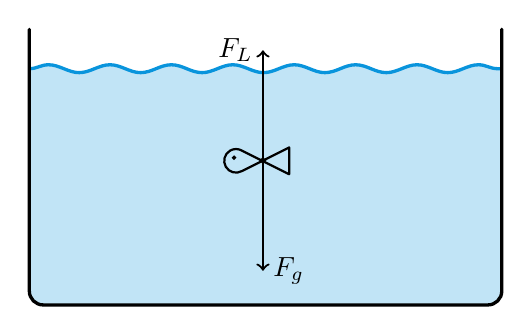
\begin{tikzpicture}[every path/.style={thick}]
            %water
            \draw[very thick, decorate, decoration={snake,amplitude=.5mm,segment length=0.78cm, post length=.1mm}, color=cyan!80!blue] (-3,-0.5) -- ++(6,0);
            \fill [color=cyan!80!blue, fill opacity=0.25] decorate [decoration={snake,amplitude=.5mm,segment length=0.78cm, post length=.1mm}] {(-3,-0.5) -- ++(6,0)} [rounded corners=5pt] -- ++(0,-3)  -- ++(-6,0) -- ++(0,3);
            %border
            \draw[very thick, rounded corners=5pt, line cap=round] (-3,0) -- ++(0,-3.5) -- ++(6,0) -- ++(0,3.5);
            %fish
            \draw[line join=round] (0.3,-1.5) -- ++(-0.6,-0.3) arc [start angle=300, end angle=60, radius=0.15cm] -- ++(0.6,-0.3) -- cycle;
            \filldraw (-0.4, -1.63) circle [radius=0.3pt];
            %forces
            \filldraw (-0.033,-1.666) circle [radius=.7pt];
            \draw[->] (-0.033,-1.666) -- ++(0,1.4) node [anchor=east] {$F_L$};
            \draw[->] (-0.033,-1.666) -- ++(0,-1.4) node [anchor=west] {$F_g$};
        \end{tikzpicture}
    \end{center}
\end{exm}
I mer generella fall behöver man dra algebraiska slutsatser. En härledning för arkimedes princip hittar du i bilaga \ref{def:arkimedes}. I praktiken är det dock enbart tre samband du bör kunna:
\begin{align*}
    \rho_{\textit{föremål}} > \rho_{\textit{vätska}} &\implies F_g > F_L \implies \text{den sjunker} \\
    \rho_{\textit{föremål}} < \rho_{\textit{vätska}} &\implies F_g < F_L \implies \text{den lyfter} \\
    \rho_{\textit{föremål}} = \rho_{\textit{vätska}} &\implies F_g = F_L \implies \text{inget händer} 
\end{align*}
Utöver dessa bör du även kunna den generella formeln för lyftkraft:
\begin{equation*}
    \tcboxmath{F_L = \rho_{\textit{vätska}} \cdot g \cdot V_{\textit{föremål}} \, \left[\mathrm{N}\right]}
\end{equation*}
Vi vet ju att $\rho V = m$ och vi vet att $mg=F_g$ alltså vi att $F_L$ motsvarar tyngden av den undanträngda vätskan.